{\let\clearpage\relax \chapter{Entwurfsmuster}\label{entwurfsmuster}}

\section{Zweck}\label{zweck}
Wiederverwendbare Vorlage zur Problemlösung, die in einem bestimmten
Zusammenhang einsetzbar ist.

\section{Abstraktion}\label{abstraktion}

\paragraph{Abstrakte Klasse}\label{abstrakte-klasse}

Wenn Methoden auf eine bestimmte Art implementiert werden müssen oder
wenn non-public Daten oder Methoden enthalten sein sollen. Dies
beeinträchtigt nicht die Möglichkeit, reine Methodenköpfe zu definieren,
die überschrieben werden müssen.

\paragraph{Interface}\label{interface}

Reine Schnittstellenbeschreibung.

\section{Erzeugungsmuster}\label{erzeugungsmuster}
Dienen der Erzeugung von Objekten. Sie entkoppeln die Konstruktion eines
Objekts von seiner Repräsentation.

\paragraph{Abstract Factory / Abstrakte Fabrik}\label{abstract-factory}

Schnittstelle zur Erzeugung einer Familie von Objekten, wobei die konkreten
Klassen der zu instanziierenden Objekte nicht näher festgelegt werden.

\paragraph{Factory / Fabrik}\label{factory}

Objekt, das durch Methodenaufruf andere Objekte erzeugt. Das zurückgegebene
Objekt ist neu und verweist nicht zwingend auf die Factory.

\paragraph{Object Pool}\label{object-pool}

Objekte, die mehrfach verwendet werden sollen, werden nur bei der ersten
Verwendung instanziiert und dann im Objektpool aufgehoben um sie
wiederverwenden zu können.

Vorteil: Reduzierter Aufwand (Zeit / Rechenleistung)

Nachteil: Erhöht Komplexität

\paragraph{Singleton}\label{singleton}

Stellt sicher, dass von einem Objekt nur eine Instanz existiert, ist in der
Regel global verfügbar.

\section{Strukturmuster}\label{strukturmuster}
Erleichtern den Entwurf von Software durch vorgefertigte Schablonen für
Beziehungen zwischen Klassen.

\paragraph{Adapter}\label{adapter}

Übersetzt eine Schnittstelle in eine andere, dadurch wird die Kommunikation von
Klassen mit inkompatiblen Schnittstellen untereinander ermöglicht.

\paragraph{Bridge}\label{bridge}

Dient zur Trennung von Implementierung und ihrer Abstraktion. So können beide
unabhängig voneinander verändert werden.
\begin{figure}[h]
	\begin{center}
		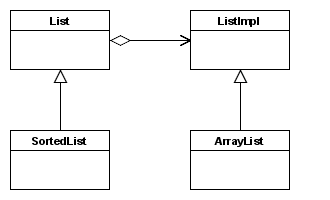
\includegraphics[width=0.2\textwidth]{images/bridge}
		\label{fig:bridge}
		\caption{Bridge}
	\end{center}
\end{figure}

\paragraph{Composition}\label{composition}

Repräsentiert Teil-Ganzes-Hierarchien, indem Objekte zu Baumstrukturen
zusammengefasst werden. Fasst in abstrakter Klasse sowohl primitive Objekte als
auch deren Behälter zusammen.
Abgesehen von der Multiplizität bei der Aggregation identisch zum Dekorierer.

Die abstrakte Klasse Knoten legt die Schnittstelle und das Verhalten der
abgeleiteten Klassen Kompositum und Blatt fest. Es wird ein Defaultverhalten für
die Kindoperationen implementiert. Die Klasse Blatt repräsentiert ein
Abschlusselement in der Baumstruktur, das keine weiteren Knoten aggregiert und
selbst immer nur Kind-Knoten sein kann. Die Klasse Kompositum repräsentiert ein
Knotenelement in der Baumstruktur, welches weitere Knoten aggregieren kann.

\paragraph{Decorator}\label{decorator}

Flexible Alternative zur Unterklassenbildung um eine Klasse nachträglich um
zusätzliche Funktionalitäten zu ergänzen.
Abgesehen von der Multiplizität bei der Aggregation identisch zum Kompositum.

\paragraph{Facade}\label{facade}

Bietet einheitliche, meist vereinfachte Schnittstelle zu einer Menge von
Schnittstellen eines Subsystems.

\paragraph{Proxy}\label{proxy}

Überträgt die Steuerung eines Objekts auf ein vorgelagertest
Stellvertreterobjekt.

\section{Verhaltensmuster}\label{verhaltensmuster}
Modellieren komplexes Verhalten der Software und erhöhen damit die Flexibilität
der Software hinsichtlich ihres Verhaltens.

\paragraph{Command}\label{command}

Kommandoobjekt kapselt einen Befehl um so zu ermöglichen, Objekte in eine
Warteschlange zu stellen, Logbucheinträge zu führen und Operationen rückgängig zu
machen.

\paragraph{Iterator}\label{iterator}

Stellt die Möglichkeit zur Verfügung, auf Elemente einer aggregierten Struktur
sequenziell zuzugreifen, ohne die Struktur zu enthüllen. Auch als Cursor
bekannt.

\paragraph{Mediator}\label{mediator}

Dienst zum Steuern des kooperativen Verhaltens von Objekten, wobei Objekte
nicht direkt kooperieren sondern über einen Vermittler.

\paragraph{Observer}\label{observer}

Beobachtetes Objekt hält eine Liste mit Beobachtern und informiert diese über
Veränderungen.

\paragraph{State}\label{state}

Kapselung zustandsabhängiger Verhaltensweisen von Objekten (vgl.
Zustandsautomat)

\paragraph{Strategy}\label{strategy}

Definiert eine Familie von Algorithmen, kapselt diese und macht sie
untereinander austauschbar. Lässt den Algorithmus unabhängig von den nutzenden
Clients variieren.

Das Strategie-Muster soll es erlauben, dass ein ganzer Algorithmus ausgetauscht
wird, um die Wiederverwendbarkeit zu steigern. Dazu soll eine Gruppe von
verschiedenen Algorithmen mit gleicher Schnittstelle definiert werden können und
jeder einzelne separat gekapselt werden, um ihn als Kapsel austauschbar zu
machen. Der jeweils zu einer bestimmten Zeit passende Algorithmus ist
auszuwählen.

\paragraph{Visitor}\label{visitor}

Repräsentiert eine Operation, die auf Elemente einer Objektstruktur ausgeführt
wird. Ermöglicht die Definition einer neuen Operation ohne die Klassen der
Elemente zu ändern, auf die es ausgeführt wird.

Beim Beobachter-Muster werden Nachrichten in beide Richtungen zwischen
BeobachterObjekt und dem beobachteten Objekt ausgetauscht. Das beobachtbare
Objekt verpflichtet den Aufrufer, eine spezielle Schnittstelle
(Callback-Schnittstelle) zu implementieren, die vom beobachtbaren Objekt
vorgegeben wird. Ändert sich der Beobachter, so hat dies keinen Einfluss auf das
beobachtbare Objekt. Dagegen wirken sich Änderungen an der
Callback-Schnittstelle oder den angebotenen Daten des beobachtbaren Objekts auf
den Beobachter aus.
